% =============================================================================
%  README.tex — Comprehensive Documentation for the Femur Mesh Processing Repo
%  Aimed at beginners: every concept, algorithm, and formula is explained
%  from scratch with intuitive descriptions.
% =============================================================================
\documentclass[12pt,a4paper]{article}

% ---- packages ---------------------------------------------------------------
\usepackage[utf8]{inputenc}
\usepackage[T1]{fontenc}
\usepackage{lmodern}
\usepackage[margin=1in]{geometry}
\usepackage{amsmath,amssymb,amsfonts}
\usepackage{graphicx}
\usepackage{xcolor}
\usepackage{hyperref}
\usepackage{listings}
\usepackage{enumitem}
\usepackage{booktabs}
\usepackage{caption}
\usepackage{tikz}
\usepackage{algorithm}
\usepackage{algorithmic}
\usepackage{fancyhdr}
\usepackage{tocloft}
\usepackage{float}
\usetikzlibrary{shapes.geometric, arrows.meta, positioning, calc}

% ---- image placeholder command ( \imgplaceholder{description}{label} ) ------
% Usage:  \imgplaceholder{Caption / suggestion for the image}{fig-label}
\newcommand{\imgplaceholder}[2]{%
    \begin{figure}[H]
    \centering
    \fcolorbox{gray!60}{gray!5}{\begin{minipage}{0.82\textwidth}
        \vspace{1.8cm}
        \begin{center}
            {\large\bfseries\color{gray!70}{[\,IMAGE PLACEHOLDER\,]}}\\[8pt]
            {\small\color{gray!55}\textit{Suggested content: #1}}
        \end{center}
        \vspace{1.8cm}
    \end{minipage}}
    \caption{#1}
    \label{fig:#2}
    \end{figure}%
}

% ---- colours & hyperlinks ---------------------------------------------------
\definecolor{codeblue}{RGB}{0,80,180}
\definecolor{codegray}{RGB}{100,100,100}
\definecolor{codegreen}{RGB}{0,120,0}
\definecolor{backcolour}{RGB}{245,245,245}
\hypersetup{
    colorlinks=true,
    linkcolor=codeblue,
    urlcolor=codeblue,
    citecolor=codeblue,
}

% ---- code listing style -----------------------------------------------------
\lstdefinestyle{pythonstyle}{
    backgroundcolor=\color{backcolour},
    commentstyle=\color{codegreen}\itshape,
    keywordstyle=\color{codeblue}\bfseries,
    stringstyle=\color{red!60!black},
    basicstyle=\ttfamily\small,
    breakatwhitespace=false,
    breaklines=true,
    captionpos=b,
    keepspaces=true,
    numbers=left,
    numbersep=8pt,
    numberstyle=\tiny\color{codegray},
    showspaces=false,
    showstringspaces=false,
    showtabs=false,
    tabsize=4,
    language=Python,
    frame=single,
    rulecolor=\color{gray!40},
}
\lstset{style=pythonstyle}

% ---- header / footer --------------------------------------------------------
\pagestyle{fancy}
\fancyhf{}
\fancyhead[L]{\textit{Femur Mesh Processing — Documentation}}
\fancyhead[R]{\thepage}
\renewcommand{\headrulewidth}{0.4pt}

% ---- title ------------------------------------------------------------------
\title{
    \vspace{-1cm}
    \textbf{Femur Mesh Processing Toolkit}\\[6pt]
    \large A Beginner-Friendly Guide to NIfTI $\rightarrow$ Watertight 3-D Mesh Conversion\\
    for Statistical Shape Modelling (SSM)
}
\author{NAAMII — Nepal Applied Mathematics and Informatics Institute}
\date{\today}

% =============================================================================
\begin{document}
\maketitle
\tableofcontents
\newpage

% =============================================================================
\section{Introduction}
% =============================================================================

\subsection{What Does This Project Do?}

This project takes \textbf{medical CT-scan images} of human femurs (thigh bones)
stored in \textbf{NIfTI format} (\texttt{.nii.gz}), and converts them into
clean, high-quality \textbf{3-D triangle meshes} saved as \texttt{.obj} files.

The meshes are:
\begin{itemize}[leftmargin=2em]
    \item \textbf{Cropped} — only the top 100\,mm of the femur (the
          \emph{proximal} end that includes the femoral head) is kept.
    \item \textbf{Watertight} — the surface is completely closed with no holes.
    \item \textbf{Separated} — left and right femurs are written to different
          folders.
\end{itemize}

\imgplaceholder{Anatomy of the proximal human femur. Label the femoral head, femoral neck, greater trochanter, lesser trochanter, and diaphysis (shaft). Indicate with a horizontal dashed line where the 100\,mm crop plane falls, roughly at the level of the lesser trochanter.}{femur-anatomy}

These meshes are used as training data for a \textbf{Statistical Shape Model
(SSM)}.  An SSM learns the average shape of a bone and how that shape varies
across a population.  Having clean, consistently cropped meshes is essential for
the SSM to work correctly.

\subsection{What Is a Statistical Shape Model (SSM)?}

Imagine you collect the femur shapes of 500 different people.  Each shape is
slightly different, but they all share a common structure (a round head, a neck,
a shaft, etc.).  An SSM captures this \emph{shared structure} mathematically.

At its core, an SSM uses \textbf{Principal Component Analysis (PCA)} on a set of
aligned shapes to find a \textbf{mean shape} $\bar{\mathbf{s}}$ and a set of
\textbf{modes of variation} $\mathbf{v}_1, \mathbf{v}_2, \ldots$\ such that any
shape $\mathbf{s}$ can be approximated as:

\begin{equation}
    \boxed{
        \mathbf{s} \;\approx\; \bar{\mathbf{s}}
        + b_1\,\mathbf{v}_1
        + b_2\,\mathbf{v}_2
        + \cdots
        + b_k\,\mathbf{v}_k
    }
    \label{eq:ssm}
\end{equation}

where $b_1, b_2, \ldots, b_k$ are scalar weights.  The first few modes usually
capture the most important variation (e.g.\ bone length, head size, neck angle).

To build an SSM, the input meshes must all:
\begin{enumerate}
    \item represent the \emph{same anatomical region} (hence the 100\,mm crop),
    \item be \emph{watertight} (for consistent correspondence), and
    \item be free of artefacts (stray fragments, missing heads, etc.).
\end{enumerate}

\noindent This toolkit ensures all three requirements.


% =============================================================================
\section{Prerequisites and Installation}
% =============================================================================

\subsection{Software Requirements}

\begin{itemize}
    \item \textbf{Python} $\geq$ 3.7
    \item \textbf{pip} (Python package manager)
\end{itemize}

\subsection{Python Dependencies}

\begin{table}[H]
\centering
\caption{Required Python packages and their roles.}
\begin{tabular}{@{}llp{7.5cm}@{}}
\toprule
\textbf{Package} & \textbf{Version} & \textbf{Purpose} \\
\midrule
\texttt{numpy}       & $\geq$ 1.21  & Fast numerical arrays and linear algebra \\
\texttt{nibabel}     & $\geq$ 3.2   & Read/write NIfTI medical image files \\
\texttt{scikit-image} & $\geq$ 0.19 & Marching Cubes algorithm (volume $\to$ mesh) \\
\texttt{trimesh}     & $\geq$ 3.10  & Triangle mesh data structure and operations \\
\texttt{pymeshfix}   & $\geq$ 0.16  & Mesh repair and hole filling \\
\texttt{pyvista}     & $\geq$ 0.37  & 3-D visualisation (used by pymeshfix) \\
\texttt{scipy}       & $\geq$ 1.7   & Scientific computing utilities \\
\texttt{shapely}     & $\geq$ 2.0   & 2-D geometry (used internally by trimesh) \\
\texttt{tqdm}        & $\geq$ 4.62  & Progress bars for batch processing \\
\bottomrule
\end{tabular}
\end{table}

\subsection{Setup Steps}

\begin{lstlisting}[language=bash,style=pythonstyle]
# 1. Clone the repository
git clone https://github.com/your-org/femur-mesh-processing.git
cd femur-mesh-processing

# 2. Create and activate a virtual environment
python -m venv venv
# Windows:
venv\Scripts\activate
# Linux / macOS:
source venv/bin/activate

# 3. Install all dependencies
pip install -r requirements.txt
\end{lstlisting}


% =============================================================================
\section{Project Structure}
% =============================================================================

% =============================================================================
\section{Dataset}
% =============================================================================

\subsection{Input Data Format}

The input data consists of femur segmentation masks stored as compressed NIfTI
files (\texttt{.nii.gz}).  Each file is a \textbf{binary 3-D volume} where
a voxel value of $1$ denotes femur bone and $0$ denotes background.
File names follow the convention:

\begin{lstlisting}[language={},basicstyle=\ttfamily\small,frame=single,numbers=none]
femur_left_msk.nii.gz     -- left femur segmentation mask
femur_right_msk.nii.gz    -- right femur segmentation mask
\end{lstlisting}

\subsection{Directory Layout}

The dataset is split into thee standard machine-learning partitions:

\begin{lstlisting}[language={},basicstyle=\ttfamily\small,frame=single,numbers=none]
Femur/
    train/  p_0001/ ... p_0372/   (each contains ct-scan/{left,right}_msk.nii.gz)
    val/    p_0001/ ... p_0047/
    test/   p_0001/ ... p_0047/
\end{lstlisting}

\begin{table}[H]
\centering
\caption{Dataset split sizes.}
\label{tab:splits}
\begin{tabular}{@{}lcccc@{}}
\toprule
\textbf{Split} & \textbf{Subjects} & \textbf{NIfTI files} & \textbf{Left} & \textbf{Right} \\
\midrule
\texttt{train} & 372 & 744 & 372 & 372 \\
\texttt{val}   &  47 &  93 &  47 &  46 \\
\texttt{test}  &  47 &  94 &  47 &  47 \\
\midrule
\textbf{Total} & 466 & 931 & 466 & 465 \\
\bottomrule
\end{tabular}
\end{table}

\subsection{Typical Volume Properties}

\begin{table}[H]
\centering
\caption{Representative properties of the input NIfTI volumes.}
\label{tab:volume-props}
\begin{tabular}{@{}ll@{}}
\toprule
\textbf{Property}    & \textbf{Typical value} \\
\midrule
Voxel spacing        & $0.4$--$0.9$\,mm (commonly $0.7\times0.7\times0.7$\,mm) \\
Volume shape         & $300$--$600 \times 300$--$600 \times 150$--$600$ voxels \\
Bone voxel value     & $1$ (binary) \quad Background: $0$ \\
File size (gzip)     & $50$--$500$\,KB \\
Initial orientation  & Varies (RAS, LPS, LAS, \ldots); always reoriented to LPS \\
\bottomrule
\end{tabular}
\end{table}

\imgplaceholder{Dataset overview: example coronal, sagittal, and axial slices of a representative femur NIfTI segmentation mask for both left and right femurs. Bone voxels should be highlighted in a distinct colour to show the binary labelling and the typical spatial extent of the femur within the scan volume.}{dataset-overview}

% =============================================================================
\section{Project Structure}
% =============================================================================

\begin{lstlisting}[language={},basicstyle=\ttfamily\small,frame=single,numbers=none]
femur-mesh-processing/
    src/
        __init__.py            # Package exports
        mesh_utils.py          # Core processing functions
  Femur/                   # Input NIfTI data
    train/
      p_0001/ct-scan/
        femur_left_msk.nii.gz
        femur_right_msk.nii.gz
      p_0002/ ...
    val/  ...
    test/ ...
  Femur_Meshes/            # Output meshes (generated)
    train/left/  train/right/
    val/left/    val/right/
    test/left/   test/right/
  process_all_crop.py      # Batch-process every file
  test_20_files.py         # Quick test on 20 files
  measure_all.py           # Measure mesh lengths
  requirements.txt
  README.md
  README.tex               # This document
\end{lstlisting}


% =============================================================================
\section{The Processing Pipeline — Overview}
% =============================================================================

Each NIfTI segmentation mask goes through ten sequential stages.
Figure~\ref{fig:pipeline} shows the flow.

\begin{figure}[H]
\centering
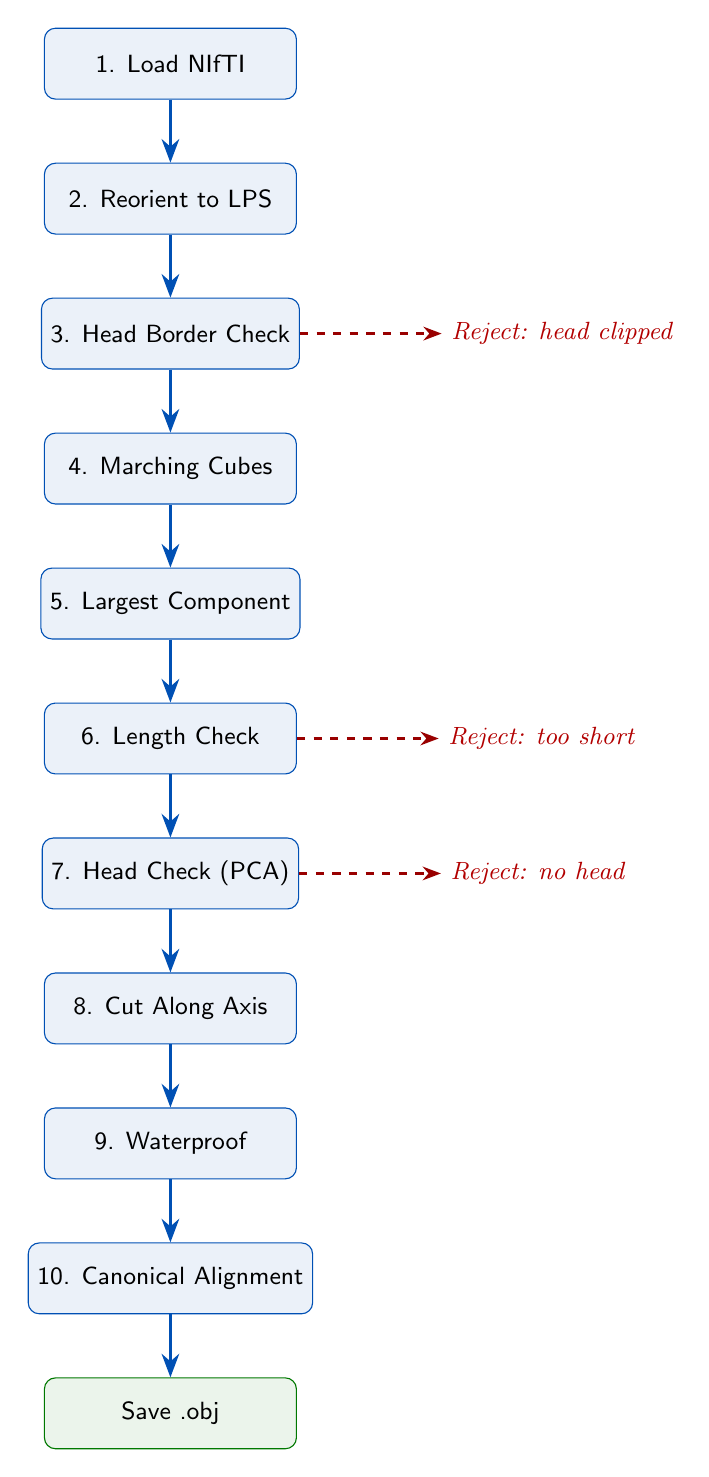
\begin{tikzpicture}[
    node distance=0.8cm and 0.5cm,
    box/.style={rectangle, draw=codeblue, fill=codeblue!8, rounded corners,
                minimum width=3.2cm, minimum height=0.9cm, align=center,
                font=\small\sffamily},
    arr/.style={-{Stealth[length=3mm]}, thick, codeblue},
]
    \node[box] (load)   {1. Load NIfTI};
    \node[box, below=of load] (lps) {2. Reorient to LPS};
    \node[box, below=of lps] (border) {3. Head Border Check};
    \node[box, below=of border] (mc) {4. Marching Cubes};
    \node[box, below=of mc] (comp) {5. Largest Component};
    \node[box, below=of comp] (len) {6. Length Check};
    \node[box, below=of len] (head) {7. Head Check (PCA)};
    \node[box, below=of head] (cut) {8. Cut Along Axis};
    \node[box, below=of cut] (water) {9. Waterproof};
    \node[box, below=of water] (align) {10. Canonical Alignment};
    \node[box, below=of align, draw=codegreen, fill=codegreen!8] (save) {Save .obj};

    \draw[arr] (load)   -- (lps);
    \draw[arr] (lps)    -- (border);
    \draw[arr] (border) -- (mc);
    \draw[arr] (mc)     -- (comp);
    \draw[arr] (comp)   -- (len);
    \draw[arr] (len)    -- (head);
    \draw[arr] (head)   -- (cut);
    \draw[arr] (cut)    -- (water);
    \draw[arr] (water)  -- (align);
    \draw[arr] (align)  -- (save);

    % Rejection arrows
    \node[right=1.8cm of border, text=red!70!black, font=\small\itshape] (rej0) {Reject: head clipped};
    \draw[-{Stealth}, thick, red!60!black, dashed] (border.east) -- (rej0.west);

    \node[right=1.8cm of len, text=red!70!black, font=\small\itshape] (rej1) {Reject: too short};
    \draw[-{Stealth}, thick, red!60!black, dashed] (len.east) -- (rej1.west);

    \node[right=1.8cm of head, text=red!70!black, font=\small\itshape] (rej2) {Reject: no head};
    \draw[-{Stealth}, thick, red!60!black, dashed] (head.east) -- (rej2.west);
\end{tikzpicture}
\caption{End-to-end mesh processing pipeline.  All volumes are first reoriented
         to LPS at stage 2 for consistent orientation.  Bones that fail quality
         checks at stages 3, 6, or 7 are rejected (not saved).  Stage~3 only
         checks the \textbf{superior face} (femoral head region) — bone
         touching other boundaries is acceptable.  All surviving
         meshes are canonically aligned at stage 10.}
\label{fig:pipeline}
\end{figure}


% =============================================================================
\section{Stage-by-Stage Explanation with Mathematics}
% =============================================================================

% -----------------------------------------------------------------------------
\subsection{Stage 1 — Loading the NIfTI File}

\subsubsection{What Is NIfTI?}

NIfTI (\textbf{N}euroimaging \textbf{I}nformatics \textbf{T}echnology
\textbf{I}nitiative) is a standard file format for storing 3-D medical images
(CT scans, MRI, etc.).  A \texttt{.nii.gz} file contains:

\begin{enumerate}
    \item A \textbf{3-D array of voxel intensities} — think of it as a 3-D grid
          of tiny cubes (voxels).  In our case the values are binary:
          1 = bone, 0 = background.
    \item A \textbf{header} with metadata, including the \emph{voxel spacing}
          $(s_x, s_y, s_z)$ in millimetres.
\end{enumerate}

\subsubsection{Voxel Spacing}

The voxel spacing tells us the \emph{physical size} of each tiny cube.
If the spacing is $(0.7, 0.7, 0.7)$\,mm, then each voxel represents a cube
of side $0.7$\,mm. This is crucial: without spacing, we would not know how big
the bone actually is.

\begin{equation}
    \text{Physical coordinate of voxel } (i,j,k) =
    \bigl(i \cdot s_x,\; j \cdot s_y,\; k \cdot s_z\bigr)
\end{equation}

\subsubsection{Code}

\begin{lstlisting}
def load_nifti(file_path):
    """Load a NIfTI file and return (volume, nifti_image)."""
    nifti_img = nib.load(file_path)     # open the file
    data = nifti_img.get_fdata()        # 3-D numpy array
    return data, nifti_img
\end{lstlisting}

The spacing is extracted later with:

\begin{lstlisting}
spacing = nifti_img.header.get_zooms()[:3]   # e.g. (0.7, 0.7, 0.7)
\end{lstlisting}


% -----------------------------------------------------------------------------
\subsection{Stage 2 — Reorient to LPS}
\label{sec:lps}

\subsubsection{The Problem: Inconsistent Volume Orientations}

CT scans are stored in NIfTI files with an \textbf{affine matrix} that maps
voxel indices $(i,j,k)$ to physical (scanner) coordinates.  Different scanners,
imaging protocols, and DICOM-to-NIfTI converters produce different
\textbf{orientation conventions}: RAS (Right-Anterior-Superior), LPS
(Left-Posterior-Superior), LAS, RPI, etc.

This means that array axis~0 might correspond to the Left-Right direction in
one scan but to the Inferior-Superior direction in another.  When we run
Marching Cubes on the raw voxel array, the resulting mesh vertices inherit this
arbitrary orientation — which is why the bones ``look too random'' when viewed
side by side.

\subsubsection{What Is LPS?}

LPS stands for \textbf{L}eft-\textbf{P}osterior-\textbf{S}uperior.  In LPS
orientation the three array axes correspond to:

\begin{center}
\begin{tabular}{cll}
    \toprule
    \textbf{Axis} & \textbf{Direction (increasing index)} & \textbf{Anatomical} \\
    \midrule
    0 & Right $\to$ Left       & L \\
    1 & Anterior $\to$ Posterior & P \\
    2 & Inferior $\to$ Superior  & S \\
    \bottomrule
\end{tabular}
\end{center}

LPS is the standard DICOM/radiological convention.  By converting every volume
to LPS \emph{before any processing}, axis~2 always runs foot-to-head, axis~0
always runs right-to-left, etc.  All downstream geometry (Marching Cubes
vertices, PCA axes, long-axis direction) is therefore consistent across scans.

\subsubsection{How It Works}

\begin{enumerate}
    \item \textbf{Canonicalise to RAS+.}  \texttt{nibabel.as\_closest\_canonical()}
          permutes and/or flips the array axes so that increasing indices
          correspond to Right, Anterior, Superior (the nibabel default).
    \item \textbf{RAS+ $\to$ LPS+.}  Flip the first two axes:
          $R \to L$ (reverse axis~0) and $A \to P$ (reverse axis~1).  Axis~2
          ($S$) is unchanged.
    \item \textbf{Update the affine.}  Negate the corresponding columns of the
          affine matrix and shift the origin so that the physical coordinates
          remain correct.
\end{enumerate}

Mathematically, if $\mathbf{A}_{\text{RAS}}$ is the $4 \times 4$ affine after
step~1, the LPS affine is:

\begin{equation}
    \boxed{
        \mathbf{A}_{\text{LPS}} =
        \mathbf{A}_{\text{RAS}} \;
        \operatorname{diag}(-1,\,-1,\,+1,\,+1)
        \; + \; \Delta
    }
    \label{eq:lps_affine}
\end{equation}

where $\Delta$ corrects the translation component so that the physical origin
maps to the same world coordinate after flipping.

\subsubsection{Code}

\begin{lstlisting}
def reorient_to_lps(nifti_img):
    # Step 1: bring to RAS+ (nibabel canonical)
    canonical = nib.as_closest_canonical(nifti_img)

    # Step 2: RAS+ -> LPS+  (flip axes 0 and 1)
    ras_data = canonical.get_fdata()
    lps_data = ras_data[::-1, ::-1, :].copy()

    # Step 3: update affine
    lps_affine = canonical.affine.copy()
    lps_affine[:3, 0] = -lps_affine[:3, 0]
    lps_affine[:3, 3] += canonical.affine[:3, 0] * (ras_data.shape[0] - 1)
    lps_affine[:3, 1] = -lps_affine[:3, 1]
    lps_affine[:3, 3] += canonical.affine[:3, 1] * (ras_data.shape[1] - 1)

    lps_img = nib.Nifti1Image(lps_data, lps_affine, canonical.header)
    spacing = tuple(float(s) for s in lps_img.header.get_zooms()[:3])
    ornt = nib.aff2axcodes(lps_affine)

    return lps_data, spacing, ornt
\end{lstlisting}

\imgplaceholder{LPS reorientation. Show the same femur voxel array in three different starting orientations (RAS, LAS, oblique), and the unified result after reorientation to LPS. Annotate the anatomical direction of each array axis before and after, and highlight that axis~2 always corresponds to Inferior$\to$Superior in LPS.}{lps-reorientation}

% -----------------------------------------------------------------------------
\subsection{Stage 3 — Head Border Check (Proximal Clipping Detection)}
\label{sec:bordercheck}

\subsubsection{Why?}

CT scans have a finite field of view.  If the patient is positioned so that
the proximal femur extends beyond the scanned region, the femoral head will
be clipped — its shape is incomplete and unusable for SSM.

However, bone voxels touching \emph{other} boundaries (e.g.\ the distal end
at the inferior face, or lateral surfaces) do \textbf{not} indicate a problem:
the distal shaft will be cropped away in Stage~8, and lateral contact is
anatomically benign.  We therefore check \textbf{only the superior face} of
the LPS-oriented volume — that is where the femoral head lives.

\subsubsection{How It Works}

After LPS reorientation (Stage~2), axis~2 runs Inferior\,$\to$\,Superior.
The femoral head sits at the \textbf{superior end} — the last slice along
axis~2:
\[
    \texttt{sup\_face} = \texttt{volume[:, :, -1]}
\]

We count the number of bone voxels on that face:
\begin{equation}
    \boxed{
        \text{clipped} =
        \begin{cases}
            \text{True}  & \text{if } \displaystyle\sum_{(i,j) \in \text{sup\_face}}
                           \mathbf{1}[\text{vol}(i,j) \geq \tau] \;\geq\; N_{\min} \\[6pt]
            \text{False} & \text{otherwise}
        \end{cases}
    }
    \label{eq:bordercheck}
\end{equation}

If $\text{clipped} = \text{True}$, the bone is rejected because the head
shape is incomplete.

\subsubsection{Code}

\begin{lstlisting}
def head_border_check(volume, threshold=0.5, min_border_voxels=10):
    bone = volume >= threshold
    sup_face = bone[:, :, -1]          # axis2_max = superior face in LPS
    count = int(sup_face.sum())
    if count >= min_border_voxels:
        return False, f"femoral head clipped at superior boundary ({count} voxels)"
    return True, "ok"
\end{lstlisting}

\imgplaceholder{Head border check. Left panel: a femur volume (side view) whose femoral head does not touch the superior boundary --- the superior face (top slice) is clean, the scan passes. Right panel: a clipped femur where the head extends to the last slice --- the superior face shows bone voxels, the scan is rejected. Annotate the boundary face and voxel count.}{border-check}

% -----------------------------------------------------------------------------
\subsection{Stage 4 — Marching Cubes: From Voxels to a Triangle Mesh}
\label{sec:mc}

\subsubsection{The Problem}

We have a 3-D binary grid (1 = bone, 0 = not bone).  We want to extract the
\emph{surface} that separates bone from non-bone as a set of triangles.

\subsubsection{The Marching Cubes Algorithm (Intuition)}

Imagine sliding a tiny cube (made of $2 \times 2 \times 2 = 8$ voxels) through
every position in the 3-D grid.  At each position we check the 8 corner values:

\begin{itemize}
    \item If a corner value $\geq$ threshold $\tau$ (default $\tau = 0.5$),
          that corner is \textbf{inside} the bone.
    \item If a corner value $<$ threshold, that corner is \textbf{outside}.
\end{itemize}

Since each corner is either inside or outside, there are $2^8 = 256$ possible
configurations.  For each configuration, a pre-computed lookup table tells us
\emph{which triangles} to create inside that cube.  The triangles are positioned
on the cube edges by \textbf{linear interpolation} between the inside and
outside corner values to find the exact surface crossing point.

\subsubsection{Mathematical Formulation}

Let $f(i,j,k)$ be the voxel value at grid position $(i,j,k)$.  For an edge
connecting two adjacent voxels $\mathbf{p}_1$ (value $v_1$) and $\mathbf{p}_2$
(value $v_2$), if $v_1$ and $v_2$ straddle the threshold $\tau$, the surface
crossing point $\mathbf{p}^*$ is:

\begin{equation}
    \boxed{
        \mathbf{p}^* = \mathbf{p}_1 + \frac{\tau - v_1}{v_2 - v_1}
        \,(\mathbf{p}_2 - \mathbf{p}_1)
    }
    \label{eq:interp}
\end{equation}

In our case the mask is binary ($v \in \{0, 1\}$), so the surface point is
always at the midpoint of the edge.

\subsubsection{Incorporating Voxel Spacing}

After the algorithm produces vertex positions in \emph{voxel index space},
each vertex $(x_v, y_v, z_v)$ is scaled by the spacing:

\begin{equation}
    \mathbf{p}_{\text{physical}} =
    \begin{pmatrix} x_v \cdot s_x \\ y_v \cdot s_y \\ z_v \cdot s_z \end{pmatrix}
\end{equation}

This ensures all distances are in millimetres.

\subsubsection{Code}

\begin{lstlisting}
def volume_to_mesh(volume, spacing, threshold=0.5):
    vertices, faces, _, _ = measure.marching_cubes(
        volume,
        level=threshold,
        spacing=tuple(float(s) for s in spacing),
        allow_degenerate=False,
    )
    return trimesh.Trimesh(vertices=vertices, faces=faces, process=False)
\end{lstlisting}

The function returns a \texttt{trimesh.Trimesh} object — a data structure that
stores a list of 3-D vertices and a list of triangular faces (each face is a
triplet of vertex indices).

\imgplaceholder{Marching Cubes reconstruction. Left: an axial slice of the binary femur segmentation volume with bone voxels in white. Centre: a zoomed $2\times2\times2$-voxel cube showing the inside/outside corner labels and the interpolated triangle placed on a crossing edge. Right: the resulting full triangulated surface mesh of the femur rendered as a shaded 3-D solid.}{marching-cubes}

% -----------------------------------------------------------------------------
\subsection{Stage 5 — Keeping Only the Largest Connected Component}

\subsubsection{Why?}

The CT segmentation mask sometimes includes small fragments — bits of the
pelvis, patella, or noise.  These appear as small disconnected ``islands'' in
the mesh.  We want only the main femur.

\subsubsection{How It Works}

A \textbf{connected component} is a maximal set of triangles where you can walk
from any triangle to any other through shared edges.  The algorithm:

\begin{enumerate}
    \item Split the mesh into connected components.
    \item Count the number of faces in each component.
    \item Keep only the component with the most faces (the main bone).
\end{enumerate}

\subsubsection{Code}

\begin{lstlisting}
def keep_largest_component(mesh):
    components = mesh.split(only_watertight=False)
    if len(components) == 1:
        return mesh
    return max(components, key=lambda c: len(c.faces))
\end{lstlisting}


% -----------------------------------------------------------------------------
\subsection{Stage 6 — Length Check (Quality Gate)}

\subsubsection{Purpose}

If the bone is shorter than the desired crop length (100\,mm), we cannot
meaningfully crop it.  Such short bones usually indicate a bad segmentation,
so we reject them.

\subsubsection{Measuring the Bone Length}

We measure the bone's \emph{anatomical length} — the length along its longest
axis.  This is done using PCA (explained in detail in Stage~5).  In brief:

\begin{enumerate}
    \item Compute the first principal component $\mathbf{v}_1$ of the vertices.
    \item Project every vertex onto $\mathbf{v}_1$.
    \item The bone length is the difference between the maximum and minimum
          projections:
\end{enumerate}

\begin{equation}
    \boxed{
        L = \max_i(\mathbf{x}_i \cdot \mathbf{v}_1)
          - \min_i(\mathbf{x}_i \cdot \mathbf{v}_1)
    }
    \label{eq:length}
\end{equation}

If $L < 100$\,mm, the bone is rejected.

\subsubsection{Code}

\begin{lstlisting}
def mesh_length_check(mesh, min_length_mm):
    verts = mesh.vertices
    centroid = verts.mean(axis=0)
    _, _, Vt = np.linalg.svd(verts - centroid, full_matrices=False)
    proj = verts @ Vt[0]
    bone_length = float(proj.max() - proj.min())

    if bone_length < min_length_mm:
        return False, f"bone too short ({bone_length:.1f} mm)", bone_length
    return True, "ok", bone_length
\end{lstlisting}


% -----------------------------------------------------------------------------
\subsection{Stage 7 — Computing the Long Axis with PCA (and Head Check)}
\label{sec:pca}

This is the most mathematically involved stage, so we build up from the basics.

\subsubsection{What Is PCA?}

\textbf{Principal Component Analysis} finds the directions along which a set of
data points varies the most.

\paragraph{Intuition.}
Imagine a cloud of points shaped like a long cigar.  PCA finds:
\begin{itemize}
    \item \textbf{PC1} — the direction of the cigar's length (most variation).
    \item \textbf{PC2} — the direction of the cigar's width (second most).
    \item \textbf{PC3} — the direction of the cigar's thickness (least).
\end{itemize}

For a femur, PC1 aligns with the long shaft — the bone's
\textbf{anatomical long axis}.

\subsubsection{Step-by-Step PCA Mathematics}

Given $n$ mesh vertices $\mathbf{x}_1, \ldots, \mathbf{x}_n \in \mathbb{R}^3$:

\paragraph{1. Centre the data.}
Compute the centroid (mean):
\begin{equation}
    \bar{\mathbf{x}} = \frac{1}{n} \sum_{i=1}^{n} \mathbf{x}_i
\end{equation}
and subtract it:
\begin{equation}
    \tilde{\mathbf{x}}_i = \mathbf{x}_i - \bar{\mathbf{x}}
\end{equation}

\paragraph{2. Form the data matrix.}
Stack the centred points as rows:
\begin{equation}
    \mathbf{X} =
    \begin{pmatrix}
        \tilde{\mathbf{x}}_1^T \\
        \tilde{\mathbf{x}}_2^T \\
        \vdots \\
        \tilde{\mathbf{x}}_n^T
    \end{pmatrix}
    \in \mathbb{R}^{n \times 3}
\end{equation}

\paragraph{3. Singular Value Decomposition (SVD).}
The SVD of $\mathbf{X}$ is:
\begin{equation}
    \boxed{
        \mathbf{X} = \mathbf{U} \, \boldsymbol{\Sigma} \, \mathbf{V}^T
    }
    \label{eq:svd}
\end{equation}

where:
\begin{itemize}
    \item $\mathbf{U} \in \mathbb{R}^{n \times 3}$ — left singular vectors
          (column-orthonormal).
    \item $\boldsymbol{\Sigma} = \operatorname{diag}(\sigma_1, \sigma_2, \sigma_3)$
          — singular values, $\sigma_1 \geq \sigma_2 \geq \sigma_3 \geq 0$.
    \item $\mathbf{V}^T \in \mathbb{R}^{3 \times 3}$ — right singular vectors
          (rows are the principal directions).
\end{itemize}

The \textbf{first row of $\mathbf{V}^T$} is the first principal component —
the direction of greatest variance.  In our code this is \texttt{Vt[0]}, and
it gives the \textbf{long axis} of the bone.

\paragraph{Relationship to the Covariance Matrix.}
PCA is equivalent to eigen-decomposing the covariance matrix $\mathbf{C}$:
\begin{equation}
    \mathbf{C} = \frac{1}{n-1}\,\mathbf{X}^T \mathbf{X}
\end{equation}
The principal components are the eigenvectors of $\mathbf{C}$, and the
eigenvalues are $\lambda_k = \sigma_k^2 / (n-1)$.  Using SVD directly on
$\mathbf{X}$ is more numerically stable.

\subsubsection{Orienting the Axis Toward the Femoral Head}
\label{sec:orient}

SVD gives an axis direction, but it could point either way (toward the head or
toward the knee).  We need it pointing toward the \textbf{proximal (head) end},
which is the \textbf{wider} end of the femur.

\paragraph{Method.}
At each end of the bone (End A and End B), we measure the
\textbf{perpendicular spread} — how much the vertices near that end fan out
sideways.  The wider end is the proximal (head + trochanter) end.

For a set of vertices $\{\mathbf{x}_i\}$ near one tip, their perpendicular
component relative to the axis $\mathbf{a}$ is:

\begin{equation}
    \mathbf{x}_i^{\perp} = \mathbf{x}_i
    - (\mathbf{x}_i \cdot \mathbf{a})\,\mathbf{a}
    \label{eq:perp}
\end{equation}

The perpendicular \textbf{RMS spread} is:

\begin{equation}
    \boxed{
        \text{spread} = \sqrt{
            \frac{1}{m} \sum_{i=1}^{m}
            \left\| \mathbf{x}_i^{\perp} - \overline{\mathbf{x}^{\perp}} \right\|^2
        }
    }
    \label{eq:spread}
\end{equation}

where $\overline{\mathbf{x}^{\perp}}$ is the mean of the perpendicular
components and $m$ is the number of vertices in the tip region.

If End B is wider than End A, the axis is flipped:
$\mathbf{a} \leftarrow -\mathbf{a}$.

\subsubsection{Code}

\begin{lstlisting}
def compute_mesh_long_axis(mesh):
    verts = mesh.vertices
    centroid = verts.mean(axis=0)
    _, _, Vt = np.linalg.svd(verts - centroid, full_matrices=False)
    axis = Vt[0]   # first principal component

    proj = verts @ axis
    end_a = verts[proj.argmax()]   # one tip
    end_b = verts[proj.argmin()]   # other tip

    def perp_spread(tip_point):
        tip_proj = float(tip_point @ axis)
        bone_len = float(proj.max() - proj.min())
        mask = np.abs(verts @ axis - tip_proj) < 0.15 * bone_len
        pts = verts[mask]
        if len(pts) < 3:
            return 0.0
        perp = pts - np.outer(pts @ axis, axis)
        return float(np.sqrt(np.mean(
            np.sum((perp - perp.mean(0))**2, axis=1)
        )))

    if perp_spread(end_b) > perp_spread(end_a):
        axis = -axis   # flip toward wider (proximal) end

    top_point = verts[(verts @ axis).argmax()]
    return axis, top_point
\end{lstlisting}


\subsubsection{Femoral Head Quality Check}
\label{sec:headcheck}

Not all segmentation masks contain the femoral head — some only have the shaft.
Shaft-only bones are useless for SSM, so we detect and reject them.

\paragraph{Anatomical Observation.}
A proper proximal femur has a distinctive width profile along its length:
\begin{itemize}
    \item \textbf{Top 10\%} (femoral head sphere) — \textbf{narrow}
    \item \textbf{10--30\%} (trochanteric region) — \textbf{wide} (flares out)
    \item \textbf{Below 30\%} (shaft) — roughly uniform width
\end{itemize}

A shaft-only bone has \emph{nearly uniform width from tip to middle}.

\paragraph{The Tip Ratio Test.}
We compute the perpendicular spread (Equation~\ref{eq:spread}) in several
10\%-wide bands from the proximal end.  Let:

\begin{align}
    \text{tip\_spread}     &= \text{spread of the top 10\%} \\
    \text{max\_top\_spread} &= \max(\text{spread of bands 1--5, i.e.\ top 50\%})
\end{align}

The \textbf{tip ratio} is:

\begin{equation}
    \boxed{
        r = \frac{\text{tip\_spread}}{\text{max\_top\_spread}}
    }
    \label{eq:tipratio}
\end{equation}

\begin{itemize}
    \item $r < 0.85$: The tip is significantly narrower than the widest part
          $\Rightarrow$ the head is present $\Rightarrow$ \textbf{PASS}.
    \item $r \geq 0.85$: The tip is nearly as wide as the widest part
          $\Rightarrow$ no head, just shaft $\Rightarrow$ \textbf{REJECT}.
\end{itemize}

\imgplaceholder{Perpendicular width profile along the femoral long axis. Plot RMS spread (mm) vs.\ normalised position from tip (0\%) to base (100\%) for two cases: (a) a complete proximal femur showing a narrow spherical tip (femoral head), a wide trochanteric peak, and a uniform shaft; (b) a shaft-only bone with a nearly flat profile. Annotate the tip ratio $r$ for both curves and mark the $r=0.85$ rejection threshold.}{width-profile}

% -----------------------------------------------------------------------------
\subsection{Stage 8 — Cutting the Bone Perpendicular to the Long Axis}

\subsubsection{Why Cut?}

Different bones have different total lengths.  To build an SSM, we need all
shapes to represent the \emph{same anatomical region}.  We keep only the top
$C = 100$\,mm (the proximal femur), which includes the femoral head, neck,
and the upper part of the shaft.

\subsubsection{The Cutting Plane}
\label{sec:cut}

The cut is made by a \textbf{plane perpendicular to the long axis}.  A plane
in 3-D is defined by:

\begin{equation}
    \mathbf{a} \cdot \mathbf{x} = d
\end{equation}

where $\mathbf{a}$ is the plane normal (our long axis) and $d$ is the signed
distance from the origin.

From the proximal tip, we measure $C$\,mm down along the axis:

\begin{equation}
    d_{\text{cut}} = (\mathbf{x}_{\text{top}} \cdot \mathbf{a}) - C
    \label{eq:cutplane}
\end{equation}

We keep all geometry where $\mathbf{x} \cdot \mathbf{a} \geq d_{\text{cut}}$
(the proximal side of the plane).

\subsubsection{Mesh Slicing}

The \texttt{trimesh} library's \texttt{slice\_mesh\_plane} function clips the
mesh at the plane.  For each triangle that straddles the plane, new vertices and
edges are created along the intersection.  This produces a clean, straight
cut face.

\subsubsection{Code}

\begin{lstlisting}
def cut_mesh_along_axis(mesh, long_axis, top_point, cut_length_mm):
    proj_top = float(top_point @ long_axis)
    cut_proj = proj_top - cut_length_mm
    plane_origin = long_axis * cut_proj

    cropped = trimesh.intersections.slice_mesh_plane(
        mesh, long_axis, plane_origin
    )
    return cropped
\end{lstlisting}

\paragraph{Key Insight.}  The mesh itself is \emph{never rotated}.  The cut
plane is aligned to the bone's own long axis, so the cut is always anatomically
straight regardless of how the bone sits in the CT scanner.

\imgplaceholder{Proximal 100\,mm crop. Left: the full femur mesh with the cutting plane visualised as a semi-transparent disc perpendicular to the anatomical long axis, 100\,mm below the femoral head apex. Right: the retained proximal segment with a clean flat cut face at the distal end. Annotate the 100\,mm measurement along the long axis.}{cutting}

% -----------------------------------------------------------------------------
\subsection{Stage 9 — Waterproofing (Mesh Repair)}

\subsubsection{The Problem}

After slicing, one end of the mesh is open — there is a hole where the cut was
made.  A ``watertight'' mesh is one where the surface is completely closed (if
you filled it with water, none would leak out).

Watertight meshes are required for:
\begin{itemize}
    \item Volume computation
    \item Consistent surface parameterisation (needed by SSMs)
    \item Many mesh-processing algorithms that assume a closed manifold
\end{itemize}

\subsubsection{How PyMeshFix Repairs a Mesh}

\texttt{pymeshfix} implements the algorithm by \emph{Attene (2010)}: ``A
lightweight approach to repairing digitized polygon meshes.''  It:

\begin{enumerate}
    \item Detects boundary edges (edges belonging to only one triangle).
    \item Fills holes by triangulating the boundary loops.
    \item Removes self-intersecting and degenerate triangles.
    \item Ensures consistent face orientation (normals point outward).
\end{enumerate}

The mathematical details of hole-filling involve computing a
\textbf{minimum-area triangulation} of each boundary polygon, then refining
it to match the local curvature.

\subsubsection{Code}

\begin{lstlisting}
def waterproof_mesh(mesh):
    verts = np.asarray(mesh.vertices, dtype=np.float64)
    faces = np.asarray(mesh.faces, dtype=np.int32)

    fixer = pymeshfix.MeshFix(verts, faces)
    fixer.repair()

    return trimesh.Trimesh(vertices=fixer.points, faces=fixer.faces)
\end{lstlisting}


% -----------------------------------------------------------------------------
\subsection{Stage 10 — Canonical Alignment}
\label{sec:align}

\subsubsection{The Problem: Every Bone Faces a Different Direction}

When a patient is placed in a CT scanner, their leg may be rotated, tilted, or
slightly bent.  Each resulting segmentation mask therefore has the femur oriented
differently in 3-D space.  Looking at the meshes side-by-side makes this obvious:
some heads point up-left, others down-right, etc.

\subsubsection{Why Na\"ive PCA on the Cut Mesh Fails}
\label{sec:naivepca_fail}

An obvious idea is to run PCA on the final mesh and use the sign of the first
principal component to determine which end is the head.  This is \textbf{unreliable}
after cutting to 100\,mm, for the following reason.

After the proximal 100\,mm is kept and the mesh is waterproofed, the
\textbf{distal (cut) end} has a large, flat circular face.
The ring of vertices on that face has substantial perpendicular spread
(they form a wide circle).  The perp-spread heuristic then \emph{mistakes the
cut end for the proximal (head) end}, and many bones end up upside-down.

\subsubsection{The Fix: Use the Pre-Cut Long Axis}

The correct long axis is already computed in Stage~5 on the \textbf{full,
uncut bone}, where the contrast between the wide trochanteric region and the
narrow shaft tip gives a reliable reading.  We simply hold on to that
vector and pass it into the alignment function, bypassing any recomputation
on the cut mesh:

\begin{lstlisting}
# Stage 5 output:
long_axis, top_point = compute_mesh_long_axis(mesh)  # full bone

# ... cut, waterproof ...

# Stage 8: pass the pre-cut axis directly
mesh = align_mesh_to_canonical_axes(mesh, long_axis=long_axis)
\end{lstlisting}

For the transverse axis (PC2) we still run SVD on the cut mesh, which is
fine because PC2 is determined by the widest transverse dimension (neck
vs.~trochanter) and is not affected by the flat cut face.

For an SSM to work, all shapes must be expressed in the \textbf{same coordinate
frame}.  Canonical alignment achieves this by rotating each mesh so that:

\begin{center}
\begin{tabular}{cll}
    \toprule
    \textbf{Axis} & \textbf{Direction} & \textbf{Anatomical meaning} \\
    \midrule
    $+Z$ & upward & long axis of the femur; femoral head at the top \\
    $+X$ & rightward & widest transverse direction (PC2) \\
    $+Y$ & forward & $Z \times X$ (right-hand rule) \\
    origin & centre & mesh centroid \\
    \bottomrule
\end{tabular}
\end{center}

\subsubsection{Step-by-Step Mathematics}

\paragraph{Step 1 — Centring.}
Translate the mesh so its centroid $\bar{\mathbf{x}}$ is at the origin:
\begin{equation}
    \tilde{\mathbf{x}}_i = \mathbf{x}_i - \bar{\mathbf{x}},
    \qquad
    \bar{\mathbf{x}} = \frac{1}{n}\sum_{i=1}^{n}\mathbf{x}_i
\end{equation}

\paragraph{Step 2 — PCA via SVD (for PC2) / use pre-cut axis (for PC1).}
If the caller supplies \texttt{long\_axis} (from Stage~5 on the full bone),
that vector is used directly as $\mathbf{p}_1$.  Otherwise a full SVD is run.
In either case the transverse axis $\mathbf{p}_2$ is taken from the SVD of
the cut mesh and Gram-Schmidt-orthogonalised against $\mathbf{p}_1$:
\begin{equation}
    \mathbf{p}_2 \leftarrow \frac{\mathbf{p}_2^{\rm raw}
    - (\mathbf{p}_2^{\rm raw} \cdot \mathbf{p}_1)\,\mathbf{p}_1}
    {\|\mathbf{p}_2^{\rm raw} - (\mathbf{p}_2^{\rm raw}\cdot\mathbf{p}_1)\,\mathbf{p}_1\|}
    \label{eq:gramschmidt}
\end{equation}

\paragraph{Step 3 — Orient $\mathbf{p}_1$ toward the proximal end.}
Using the perpendicular-spread heuristic from Section~\ref{sec:orient}, flip
$\mathbf{p}_1$ if necessary so it points toward the wider (head) end:
\begin{equation}
    \mathbf{p}_1 \leftarrow
    \begin{cases}
        \mathbf{p}_1  & \text{if spread}(\text{end}_A) > \text{spread}(\text{end}_B) \\
        -\mathbf{p}_1 & \text{otherwise}
    \end{cases}
\end{equation}

\paragraph{Step 4 — Fix the sign of $\mathbf{p}_2$.}
PCA gives the \emph{direction} of the second principal axis but not its sign.  We
choose the sign deterministically:
\begin{equation}
    \mathbf{p}_2 \leftarrow
    \begin{cases}
        \mathbf{p}_2  & \text{if } p_{2,x} \geq 0 \\
        -\mathbf{p}_2 & \text{if } p_{2,x} < 0
    \end{cases}
\end{equation}
(i.e.\ the first component of $\mathbf{p}_2$ is always non-negative.)

\paragraph{Step 5 — Right-handed third axis.}
\begin{equation}
    \mathbf{p}_3 = \frac{\mathbf{p}_2 \times \mathbf{p}_1}
                         {\|\mathbf{p}_2 \times \mathbf{p}_1\|}
\end{equation}

\paragraph{Step 6 — Build the rotation matrix.}
Stack the canonical\,$\to$\,original mappings as rows:
\begin{equation}
    \boxed{
        \mathbf{R} =
        \begin{pmatrix}
            \mathbf{p}_2^T \\
            \mathbf{p}_3^T \\
            \mathbf{p}_1^T
        \end{pmatrix}
        \in \mathbb{R}^{3 \times 3}
    }
    \label{eq:rotmat}
\end{equation}
$\mathbf{R}$ is an \emph{orthogonal} matrix ($\mathbf{R}^{-1} = \mathbf{R}^T$)
because its rows are mutually orthonormal unit vectors.

\paragraph{Verification.}
\begin{align}
    \mathbf{R}\,\mathbf{p}_1 &= (0,\,0,\,1)^T \quad [\,+Z\,]\\
    \mathbf{R}\,\mathbf{p}_2 &= (1,\,0,\,0)^T \quad [\,+X\,]\\
    \mathbf{R}\,\mathbf{p}_3 &= (0,\,1,\,0)^T \quad [\,+Y\,]
\end{align}

\paragraph{Step 7 — Apply the rotation.}
The aligned vertex position is obtained by multiplying the centred vertex by
$\mathbf{R}^T$ (\texttt{numpy} convention: row-vectors $\times$ matrix):
\begin{equation}
    \boxed{
        \mathbf{x}_i^{\text{aligned}} = \mathbf{R}\,(\mathbf{x}_i - \bar{\mathbf{x}})
    }
    \label{eq:aligned}
\end{equation}

In code this is written as:
\texttt{aligned\_verts = verts\_c @ R.T}
because NumPy stores row-vectors, so the right multiplication by $\mathbf{R}^T$
equals the column-vector formula $\mathbf{R}\tilde{\mathbf{x}}_i$.

\subsubsection{Why Not Use Procrustes / ICP?}

\textbf{Procrustes Analysis} and \textbf{Iterative Closest Point (ICP)} align
one shape \emph{to another reference shape} — they minimise the sum of squared
distances between corresponding points across all shapes simultaneously.  This
gives a more accurate pairwise alignment but requires all meshes to have the
same number of vertices (or a correspondence map).

Our PCA-based alignment is \textbf{intrinsic} — each bone is aligned
independently using only its own geometry.  This is:
\begin{itemize}
    \item Faster (no iteration, no correspondence)
    \item Sufficient for making all meshes face the same direction
    \item A good pre-processing step before running full Procrustes/ICP
\end{itemize}

\subsubsection{Code}

\begin{lstlisting}
def align_mesh_to_canonical_axes(mesh):
    verts    = np.array(mesh.vertices, dtype=np.float64)
    centroid = verts.mean(axis=0)
    verts_c  = verts - centroid                  # step 1: centre

    _, _, Vt = np.linalg.svd(verts_c, full_matrices=False)
    pc1 = Vt[0].copy()                           # step 2: long axis
    pc2 = Vt[1].copy()                           # widest transverse

    # step 3: orient pc1 toward wider (proximal) end
    # ... (same perp_spread logic as compute_mesh_long_axis)
    if _perp_spread(end_b) > _perp_spread(end_a):
        pc1 = -pc1

    # step 4: fix pc2 sign deterministically
    if pc2[0] < 0:
        pc2 = -pc2

    # step 5: right-handed pc3
    pc3 = np.cross(pc2, pc1)
    pc3 /= np.linalg.norm(pc3)

    # step 6: rotation matrix
    R = np.array([pc2, pc3, pc1])    # shape (3, 3)

    # step 7: rotate
    aligned_verts = verts_c @ R.T
    return trimesh.Trimesh(vertices=aligned_verts, faces=mesh.faces)
\end{lstlisting}

\imgplaceholder{Canonical alignment result. Left panel: six femur meshes after the 100\,mm crop, each in its original CT-scanner orientation (heads pointing in arbitrary directions due to patient positioning). Right panel: the same six meshes after canonical alignment --- all heads pointing upward along $+Z$, centred at the origin. Label the $X$, $Y$, $Z$ axes on at least one aligned mesh.}{canonical-alignment}

% =============================================================================
\section{Key Mathematical Concepts — Summary}
% =============================================================================

\begin{table}[H]
\centering
\renewcommand{\arraystretch}{1.4}
\caption{Summary of mathematical concepts used in the pipeline.}
\begin{tabular}{@{}p{3.5cm}p{10cm}@{}}
\toprule
\textbf{Concept} & \textbf{Where and How It Is Used} \\
\midrule
\textbf{Voxel Spacing} &
    Converts array indices to millimetres.
    $\mathbf{p}_{\text{mm}} = (i \cdot s_x,\; j \cdot s_y,\; k \cdot s_z)$. \\

\textbf{LPS Reorientation} &
    Permutes and flips volume axes so that axis~0 = Left, axis~1 = Posterior,
    axis~2 = Superior (Eq.~\ref{eq:lps_affine}).  Ensures all scans share
    the same physical axis layout before meshing. \\

\textbf{Border Check} &
    Counts bone voxels on the \textbf{superior face} (axis2\_max) of the
    LPS-oriented volume (Eq.~\ref{eq:bordercheck}).
    If $\geq N_{\min}$ bone voxels are found, the femoral head is clipped
    and the sample is rejected.  Other boundaries are ignored. \\

\textbf{Marching Cubes} &
    Extracts the bone surface from the binary volume.
    Uses a threshold $\tau$ and linear interpolation
    (Eq.~\ref{eq:interp}). \\

\textbf{Connected Components} &
    Graph-based splitting of the mesh.
    Keeps the largest piece (the femur), discards noise. \\

\textbf{PCA / SVD} &
    Finds the bone's long axis (Eq.~\ref{eq:svd}).
    The first right singular vector $\mathbf{v}_1$ is the direction
    of maximum variance → the shaft direction. \\

\textbf{Perpendicular Spread} &
    Measures how ``wide'' the bone is at a given slice
    (Eqs.~\ref{eq:perp}--\ref{eq:spread}).
    Used to orient the axis and detect missing heads. \\

\textbf{Tip Ratio} &
    $r = \text{tip\_spread} / \text{max\_top\_spread}$
    (Eq.~\ref{eq:tipratio}).
    $r < 0.85$ → head present; $r \geq 0.85$ → shaft only. \\

\textbf{Plane Equation} &
    $\mathbf{a} \cdot \mathbf{x} = d$ defines the cutting plane
    (Eq.~\ref{eq:cutplane}).
    Perpendicular to the long axis, $C$\,mm from the proximal tip. \\

\textbf{Hole Filling} &
    Minimum-area triangulation of boundary loops.
    Produces a watertight manifold surface. \\
\bottomrule
\end{tabular}
\end{table}


% =============================================================================
\section{The Full Pipeline Function}
% =============================================================================

The function \texttt{process\_nifti\_to\_mesh()} in \texttt{src/mesh\_utils.py}
chains all ten stages together:

\begin{lstlisting}
def process_nifti_to_mesh(input_path, output_path, threshold=0.5,
                          crop_length_mm=100.0, skip_bad=True,
                          verbose=True, align=True,
                          min_border_voxels=10):
    # Stage 1: Load NIfTI
    volume, nifti_img = load_nifti(input_path)

    # Stage 2: Reorient to LPS
    volume, spacing, ornt = reorient_to_lps(nifti_img)

    # Stage 3: Head border check (reject clipped proximal end)
    if skip_bad:
        ok, reason = head_border_check(
            volume, threshold=threshold,
            min_border_voxels=min_border_voxels)
        if not ok:
            return None, reason   # REJECTED

    # Stage 4: Marching cubes
    mesh = volume_to_mesh(volume, spacing, threshold)

    # Stage 5: Keep largest connected component
    mesh = keep_largest_component(mesh)

    # Stage 6: Length check
    if skip_bad and crop_length_mm is not None:
        ok, reason, bone_length = mesh_length_check(mesh, crop_length_mm)
        if not ok:
            return None, reason   # REJECTED

    # Stage 7: PCA long axis + head check
    long_axis, top_point = compute_mesh_long_axis(mesh)
    if skip_bad:
        ok, reason = head_check(mesh, long_axis)
        if not ok:
            return None, reason   # REJECTED

    # Stage 8: Cut perpendicular to long axis
    if crop_length_mm is not None:
        proj = mesh.vertices @ long_axis
        bone_len = proj.max() - proj.min()
        if bone_len > crop_length_mm:
            mesh = cut_mesh_along_axis(mesh, long_axis,
                                       top_point, crop_length_mm)

    # Stage 9: Waterproof
    mesh = waterproof_mesh(mesh)

    # Stage 10: Canonical alignment (all bones face the same direction)
    if align:
        mesh = align_mesh_to_canonical_axes(mesh, long_axis=long_axis)

    # Save
    mesh.export(output_path)
    return mesh, None   # success, no rejection reason
\end{lstlisting}

\paragraph{Returns.}
The function returns a tuple \texttt{(mesh, reason)}:
\begin{itemize}
    \item \texttt{mesh}: \texttt{trimesh.Trimesh} if successful, \texttt{None} if rejected
    \item \texttt{reason}: rejection reason string (\texttt{str}) if rejected,
          \texttt{None} if successful
\end{itemize}

\paragraph{Parameters.}
\begin{itemize}
    \item \texttt{input\_path}: path to the \texttt{.nii.gz} segmentation mask.
    \item \texttt{output\_path}: where to save the \texttt{.obj} mesh.
    \item \texttt{threshold}: Marching Cubes iso-value (default 0.5 for binary masks).
    \item \texttt{crop\_length\_mm}: millimetres to keep from the proximal end
          (default 100).
    \item \texttt{skip\_bad}: if \texttt{True}, reject bones that fail quality
          checks (border, length, head).
    \item \texttt{verbose}: print step-by-step progress.
    \item \texttt{align}: if \texttt{True} (default), apply canonical alignment
          after waterproofing so all output meshes share the same coordinate
          frame ($+Z$ = head-up long axis, $+X$ = widest transverse, centred at
          the origin).  Set to \texttt{False} to keep the original scanner
          orientation.
    \item \texttt{min\_border\_voxels}: minimum number of bone voxels on the
          \textbf{superior} volume boundary face to count as clipped (default
          10).  Only the superior face is checked because that is where the
          femoral head is located in LPS orientation.
\end{itemize}


% =============================================================================
\section{Batch Processing Scripts}
% =============================================================================

\subsection{\texttt{process\_all\_crop.py} — Full Dataset}

Processes every \texttt{.nii.gz} file across \texttt{train/}, \texttt{val/},
and \texttt{test/} splits.

\begin{lstlisting}[language=bash,style=pythonstyle]
python process_all_crop.py
\end{lstlisting}

\paragraph{Output layout:}
\begin{lstlisting}[language={},basicstyle=\ttfamily\small,frame=single,numbers=none]
Femur_Meshes/
  train/left/femur_001.obj  ...  train/right/femur_001.obj  ...
  val/left/   ...                val/right/   ...
  test/left/  ...                test/right/  ...
\end{lstlisting}

Each file is named sequentially (\texttt{femur\_001.obj},
\texttt{femur\_002.obj}, \ldots) within its split and side.

\subsection{\texttt{test\_20\_files.py} — Quick Test (20 files)}

Processes the first 10 left and 10 right femurs for a quick sanity check.

\begin{lstlisting}[language=bash,style=pythonstyle]
python test_20_files.py
\end{lstlisting}

Output is written to \texttt{output\_test\_20/left/} and
\texttt{output\_test\_20/right/}.

\subsection{\texttt{measure\_all.py} — Measure Mesh Lengths}

After processing, you can verify that all meshes are the expected length:

\begin{lstlisting}[language=bash,style=pythonstyle]
python measure_all.py
\end{lstlisting}

This loads every \texttt{.obj} file, computes the Z-extent of the vertices,
and prints a summary (min, max, average length).


% =============================================================================
\section{Understanding the Data Flow}
% =============================================================================

To make things concrete, here is a numeric example of what happens to a single
bone.

\begin{enumerate}
    \item \textbf{Input}: \texttt{femur\_left\_msk.nii.gz}
          — a $512 \times 512 \times 400$ binary volume with spacing
          $(0.7, 0.7, 0.7)$\,mm.

    \item \textbf{Reorient to LPS}: The volume's affine indicates it was stored
          in RAS+ orientation.  The array axes are permuted and flipped so that
          axis~0 = Left, axis~1 = Posterior, axis~2 = Superior.  Shape may
          change (axes are reordered), spacing is preserved.

    \item \textbf{Border Check}: The six boundary faces of the volume are
          inspected.  The \textbf{superior face} (axis2\_max, where the
          femoral head is) contains $< 10$ bone voxels $\Rightarrow$
          the head is not clipped $\Rightarrow$ passes.  Bone touching
          other boundaries (e.g.\ the distal end) is acceptable.

    \item \textbf{After Marching Cubes}: $\approx$\,25\,000 vertices and
          $\approx$\,50\,000 faces.  The mesh is in mm coordinates (vertices
          range from $0$ to $512 \times 0.7 = 358.4$\,mm along each axis
          where the bone exists).

    \item \textbf{After Largest Component}: same mesh if there was only one
          piece, or slightly smaller if fragments were removed.

    \item \textbf{Length Check}: PCA finds the long axis.  Projecting all
          vertices gives a bone length of, say, $L = 320$\,mm.
          Since $320 > 100$, the bone passes.

    \item \textbf{Head Check}: The tip ratio is, say, $r = 0.55 < 0.85$
          $\Rightarrow$ the head is present.

    \item \textbf{After Cutting at 100\,mm}: The mesh is trimmed to the top
          100\,mm.  Now $\approx$\,8\,000 vertices and $\approx$\,16\,000 faces.

    \item \textbf{After Waterproofing}: The cut hole is filled.  The mesh is
          watertight.  Saved as \texttt{femur\_001.obj}.
\end{enumerate}


% =============================================================================
\section{Glossary}
% =============================================================================

% =============================================================================
\section{Results and Processing Statistics}
% =============================================================================

\subsection{Pipeline Run Summary}

Running \texttt{process\_all\_crop.py} on the complete dataset of 931 NIfTI
files produces output similar to the following.  Skipped files are listed with
their rejection reason so each case can be manually reviewed:

\begin{lstlisting}[language={},basicstyle=\ttfamily\small,frame=single,numbers=none]
Found 931 files across ['train', 'val', 'test']
Crop: 100.0 mm | Quality filter: True
Output: Femur_Meshes
======================================================================
train: 100%|======================| 744/744 [02:07<00:00, 5.8it/s]
    SKIP (p_0010/.../femur_left):  bone too short (96.5 mm < 100 mm)
    SKIP (p_0021/.../femur_right): femoral head clipped (1508 voxels)
    SKIP (p_0088/.../femur_right): femoral head missing (ratio >= 0.85)
    ...
    train: left=352  right=360
val: 100%|==========================| 93/93 [00:15<00:00, 6.2it/s]
    val:   left=45   right=43
test: 100%|=========================| 94/94 [00:14<00:00, 6.7it/s]
    test:  left=46   right=45
======================================================================
Done.  saved=891  skipped=38  failed=2  total=931
Output: Femur_Meshes
======================================================================
\end{lstlisting}

\subsection{Rejection Breakdown}

Quality checks at stages 3, 6, and 7 filter out bones that are unusable for
statistical shape modelling.  Table~\ref{tab:rejections} summarises the typical
causes and counts across the full dataset:

\begin{table}[H]
\centering
\caption{Typical rejection causes and frequencies.}
\label{tab:rejections}
\renewcommand{\arraystretch}{1.35}
\begin{tabular}{@{}p{5.2cm}cp{6.2cm}@{}}
\toprule
\textbf{Rejection reason} & \textbf{Approx.\ count} & \textbf{Root cause} \\
\midrule
Femoral head clipped at\newline superior boundary &
        $\sim$15 &
        CT field of view too small; the head extends beyond the superior edge
        of the scanned volume (Stage~3). \\
\addlinespace
Bone too short ($L < 100$\,mm) &
        $\sim$20 &
        Incomplete segmentation covering only the distal shaft, or a short scan
        range (Stage~6). \\
\addlinespace
Femoral head missing\newline (tip ratio $r \geq 0.85$) &
        $\sim$3 &
        Shaft-only annotation; the femoral head was not labelled in this mask
        (Stage~7). \\
\addlinespace
Processing failure (exception) &
        $\leq$2 &
        Rare: corrupted file, all-zero volume, or numerical instability. \\
\bottomrule
\end{tabular}
\end{table}

\subsection{Output Mesh Properties}

Every mesh that passes all quality checks shares the following standardised
geometric properties after canonical alignment:

\begin{table}[H]
\centering
\caption{Geometric properties of the final processed output meshes.}
\label{tab:output-properties}
\begin{tabular}{@{}ll@{}}
\toprule
\textbf{Property}        & \textbf{Value} \\
\midrule
Crop length (Z-extent)   & $100.0$\,mm (identical for all meshes) \\
Coordinate origin        & Mesh centroid \\
Long axis ($+Z$)         & Proximal femoral direction; femoral head at maximum $+Z$ \\
Transverse axis ($+X$)   & Widest cross-sectional direction (PC2 of the cut mesh) \\
Third axis ($+Y$)        & $\mathbf{p}_1 \times \mathbf{p}_2$ (right-hand rule) \\
Watertight               & Yes (all holes filled by \texttt{pymeshfix}) \\
Typical vertex count     & $5{,}000$--$15{,}000$ \\
Typical face count       & $10{,}000$--$30{,}000$ \\
File format              & Wavefront OBJ (\texttt{.obj}) \\
Units                    & Millimetres \\
\bottomrule
\end{tabular}
\end{table}

\subsection{Visual Results}

\imgplaceholder{Mosaic of aligned femur meshes: a $4\times4$ grid showing 8 left and 8 right output meshes from the test set, all in canonical orientation (femoral head at top, long axis along $+Z$). This illustrates the geometric consistency produced by the pipeline across patients with diverse bone sizes and original scanner orientations.}{result-mosaic}

\imgplaceholder{Input-to-output comparison for three representative patients: a three-column panel where Column~1 shows a coronal slice of the raw NIfTI segmentation, Column~2 shows the full marching-cubes mesh before cropping (original CT orientation), and Column~3 shows the final 100\,mm cropped and canonically aligned mesh. Highlight the consistent head-up orientation and the clean flat cut face.}{result-comparison}

\imgplaceholder{Rejected-sample examples: three rows, one per rejection category. Row~1: femoral head clipped at the superior boundary (show the NIfTI slice with the head cut off and the exact rejection message). Row~2: bone too short (show the full mesh with its measured length $< 100$\,mm annotated). Row~3: shaft-only segmentation with tip ratio $r \geq 0.85$ (show the mesh and its flat width profile). Each row should include the pipeline's printed rejection message.}{rejected-samples}

% =============================================================================
\section{Glossary}
% =============================================================================

\begin{description}[leftmargin=3cm,style=nextline]
        \item[CT scan]
                Computed Tomography — a 3-D X-ray image of the body.

    \item[NIfTI]
        Neuroimaging Informatics Technology Initiative — a standard file format
        for 3-D medical images (\texttt{.nii} or \texttt{.nii.gz}).

    \item[Voxel]
        ``Volume pixel'' — a single cell in a 3-D grid, the 3-D analogue of a
        pixel.

    \item[Segmentation mask]
        A volume where each voxel is labelled (e.g.\ 1 = bone, 0 = background).

    \item[Triangle mesh]
        A surface representation consisting of vertices (3-D points) and faces
        (triangles connecting three vertices each).

    \item[Watertight]
        A mesh whose surface is completely closed — every edge is shared by
        exactly two triangles.

    \item[Marching Cubes]
        An algorithm that extracts a surface mesh from a 3-D scalar field at a
        given threshold value.

    \item[PCA]
        Principal Component Analysis — finds the axes of maximum variance in a
        point cloud.

    \item[SVD]
        Singular Value Decomposition — a matrix factorisation
        $\mathbf{X} = \mathbf{U}\boldsymbol{\Sigma}\mathbf{V}^T$ used to
        compute PCA.

    \item[Proximal]
        (Anatomy) Closer to the centre of the body.  For the femur, the
        proximal end has the femoral head that fits into the hip socket.

    \item[Distal]
        (Anatomy) Farther from the centre of the body.  For the femur, the
        distal end is near the knee.

    \item[Femoral head]
        The ball-shaped top of the femur that articulates with the pelvis.

    \item[Greater trochanter]
        A bony prominence near the top of the femur, lateral to the neck.
        It makes the proximal end of the bone wider.

    \item[OBJ]
        Wavefront OBJ — a simple text-based 3-D mesh file format.

    \item[SSM]
        Statistical Shape Model — a model that captures the mean shape and
        principal modes of shape variation across a population.
\end{description}


% =============================================================================
\section{Troubleshooting}
% =============================================================================

\begin{enumerate}
    \item \textbf{ImportError: No module named `nibabel`}\\
          Run \texttt{pip install -r requirements.txt} inside your virtual
          environment.

    \item \textbf{File not found errors}\\
          Ensure the \texttt{Femur/} directory exists and contains the expected
          \texttt{train/val/test} subfolders with \texttt{.nii.gz} files.

    \item \textbf{Memory errors with large files}\\
          The 100\,mm cropping significantly reduces mesh size.
          If you still run out of memory, process files one at a time.

    \item \textbf{Many bones rejected}\\
          Check your segmentation masks.  Common causes: incomplete
          segmentation (shaft only), very noisy masks, or wrong label values.

    \item \textbf{Many bones rejected by head border check}\\
          The CT scan field of view may be too small superiorly, cutting off
          the femoral head.  Inspect the NIfTI volumes to confirm.  You can
          raise \texttt{min\_border\_voxels} if single-voxel noise at the
          superior boundary is causing false positives.
\end{enumerate}


% =============================================================================
\section{References}
% =============================================================================

\begin{enumerate}
    \item Lorensen, W.\,E.\ and Cline, H.\,E.\ (1987).
          ``Marching Cubes: A high resolution 3D surface construction algorithm.''
          \textit{ACM SIGGRAPH Computer Graphics}, 21(4), 163--169.

    \item Attene, M.\ (2010).
          ``A lightweight approach to repairing digitized polygon meshes.''
          \textit{The Visual Computer}, 26(11), 1393--1406.

    \item Cootes, T.\,F., Taylor, C.\,J., Cooper, D.\,H., and Graham, J.\ (1995).
          ``Active Shape Models — Their Training and Application.''
          \textit{Computer Vision and Image Understanding}, 61(1), 38--59.

    \item Golub, G.\,H.\ and Van Loan, C.\,F.\ (2013).
          \textit{Matrix Computations}, 4th edition.  Johns Hopkins University
          Press.  (Chapter 2: SVD.)

    \item NIfTI format specification:
          \url{https://nifti.nimh.nih.gov/}

    \item \texttt{trimesh} documentation:
          \url{https://trimesh.org/}

    \item \texttt{pymeshfix} documentation:
          \url{https://pymeshfix.pyvista.org/}
\end{enumerate}


% =============================================================================
\section*{License}
% =============================================================================

This project is released under the \textbf{MIT License}.
See the \texttt{LICENSE} file for details.

\end{document}
